\documentclass[a4paper,
fontsize=11pt,
%headings=small,
oneside,
numbers=noperiodatend,
parskip=half-,
bibliography=totoc,
final
]{scrartcl}

\usepackage{synttree}
\usepackage{graphicx}
\setkeys{Gin}{width=.8\textwidth} %default pics size

\graphicspath{{./plots/}}
\usepackage[ngerman]{babel}
\usepackage[T1]{fontenc}
%\usepackage{amsmath}
\usepackage[utf8x]{inputenc}
\usepackage [hyphens]{url}
\usepackage{booktabs} 
\usepackage[left=2.4cm,right=2.4cm,top=2.3cm,bottom=2cm,includeheadfoot]{geometry}
\usepackage{eurosym}
\usepackage{multirow}
\usepackage[ngerman]{varioref}
\setcapindent{1em}
\renewcommand{\labelitemi}{--}
\usepackage{paralist}
\usepackage{pdfpages}
\usepackage{lscape}
\usepackage{float}
\usepackage{acronym}
\usepackage{eurosym}
\usepackage[babel]{csquotes}
\usepackage{longtable,lscape}
\usepackage{mathpazo}
\usepackage[normalem]{ulem} %emphasize weiterhin kursiv
\usepackage[flushmargin,ragged]{footmisc} % left align footnote
\usepackage{ccicons} 
\setcapindent{0pt} % no indentation in captions

%%%% fancy LIBREAS URL color 
\usepackage{xcolor}
\definecolor{libreas}{RGB}{112,0,0}

\usepackage{listings}

\urlstyle{same}  % don't use monospace font for urls

\usepackage[fleqn]{amsmath}

%adjust fontsize for part

\usepackage{sectsty}
\partfont{\large}

%Das BibTeX-Zeichen mit \BibTeX setzen:
\def\symbol#1{\char #1\relax}
\def\bsl{{\tt\symbol{'134}}}
\def\BibTeX{{\rm B\kern-.05em{\sc i\kern-.025em b}\kern-.08em
    T\kern-.1667em\lower.7ex\hbox{E}\kern-.125emX}}

\usepackage{fancyhdr}
\fancyhf{}
\pagestyle{fancyplain}
\fancyhead[R]{\thepage}

% make sure bookmarks are created eventough sections are not numbered!
% uncommend if sections are numbered (bookmarks created by default)
% \makeatletter
% \renewcommand\@seccntformat[1]{}
% \makeatother


\usepackage{hyperxmp}
\usepackage[colorlinks, linkcolor=black,citecolor=black, urlcolor=libreas,
breaklinks= true,bookmarks=true,bookmarksopen=true]{hyperref}
\usepackage{breakurl}

%meta
%meta

\fancyhead[L]{K. Leyrer\\ %author
LIBREAS. Library Ideas, 35 (2019). % journal, issue, volume.
\href{http://nbn-resolving.de/}
{}} % urn 
% recommended use
%\href{http://nbn-resolving.de/}{\color{black}{urn:nbn:de...}}
\fancyhead[R]{\thepage} %page number
\fancyfoot[L] {\ccLogo \ccAttribution\ \href{https://creativecommons.org/licenses/by/4.0/}{\color{black}Creative Commons BY 4.0}}  %licence
\fancyfoot[R] {ISSN: 1860-7950}

\title{\LARGE{Zur Unmöglichkeit eines neutralen Bibliotheksangebots}}% title
\author{Katharina Leyrer} % author

\setcounter{page}{1}

\hypersetup{%
      pdftitle={Zur Unmöglichkeit eines neutralen Bibliotheksangebots},
      pdfauthor={Katharina Leyrer},
      pdfcopyright={CC BY 4.0 International},
      pdfsubject={LIBREAS. Library Ideas, 35 (2019).},
      pdfkeywords={Bestandsaufbau, Collection Bias, Intermediary Effects Modells},
      pdflicenseurl={https://creativecommons.org/licenses/by/4.0/},
      pdfcontacturl={http://libreas.eu},
      baseurl={http://libreas.eu},
      pdflang={de},
      pdfmetalang={de}
     }



\date{}
\begin{document}

\maketitle
\thispagestyle{fancyplain} 

%abstracts

%body
In der Diskussion um die Bereitstellung von Literatur rechter Verlage in
Bibliotheken wird argumentiert, Bibliotheken seien zu weltanschaulicher
Neutralität verpflichtet: \enquote{Prinzipiell unterliegen Bibliotheken,
bei entsprechender Trägerschaft, als öffentliche beziehungsweise
staatlich geförderte Einrichtungen, selbstverständlich dem
Neutralitätsgebot, welches sich unter anderem von dem im Grundgesetz
(Art. 3 I GG)
formulierten allgemeinen Gleichheitsgrundrecht ableitet} (Redaktion LIBREAS 2018;
vgl. auch Schiffler 2018). Dies suggeriert jedoch, dass Bibliotheken
prinzipiell zu einer solchen Neutralität in der Lage sind -- ohne zu
benennen, wie diese Neutralität aussehen, realisiert und gewährleistet
werden kann. Dieser Beitrag hinterfragt daher, ob ein neutrales
Bibliotheksangebot überhaupt möglich ist.

Dazu wird zunächst der aktuelle Forschungsstand zu Auswahlentscheidungen
und Verzerrungen in der Erwerbungsarbeit von Bibliotheken
zusammengefasst. Daraufhin werden Modelle aus der Selektionsforschung im
Internet-Kontext als Ausgangspunkt herangezogen, um zu zeigen, welche
Faktoren den Bestandsaufbau in Bibliotheken beeinflussen. Anhand dieser
Einflussfaktoren wird diskutiert, inwiefern Neutralität in der
Bibliotheksarbeit gewährleistet werden kann.

\hypertarget{collection-bias-eine-forschungsluxfccke}{%
\section{Collection Bias -- eine
Forschungslücke}\label{collection-bias-eine-forschungsluxfccke}}

In seinem Aufsatz \enquote{Collection Development and the Psychology of
Bias} macht Brian Quinn 2012 deutlich, dass Bibliotheksbestände immer
durch die Vorlieben und Werte der Erwerbungsbibliothekar*innen verzerrt
sind. Verschiedene Studien zu einem solchen \enquote{collection bias} --
die allerdings aus den 1990er Jahren und den USA beziehungsweise Kanada
stammen -- liefern dafür Belege: Eine Studie in Kalifornien untersuchte
1995 den Bestand von 580 Wissenschaftlichen Bibliotheken zum Thema
Abtreibung, indem das Vorhandensein von jeweils acht pro-choice und acht
pro-life Büchern überprüft wurde. Dabei wurde deutlich, dass die
untersuchten Bibliotheken mit dreimal höherer Wahrscheinlichkeit
pro-choice-Literatur in ihrem Bestand hatten als pro-life-Bücher. Dies
könnte in \enquote{precensorship} begründet sein, also \enquote{the
practice of collection development librarians excluding books from the
collection as a result of conscious or subconscious bias that may be
related to social, political, or personal views} (Quinn 2012, S. 278).
Nicht nur im Bezug auf bestimmte Themen, sondern auch auf Verlage wurden
Verzerrungen belegt: So befand eine Studie in kanadischen
Wissenschaftlichen Bibliotheken, dass diese einen großen Anteil der
Zeitschriften von großen Verlagsunternehmen, aber nur etwa die Hälfte
der von kleineren Verlagen veröffentlichten Zeitschriften abonniert
hatten (Quinn 2012). Diese Studien machen deutlich: Von einer
Neutralität in der Erwerbungsarbeit in Bibliotheken kann nicht ohne
Weiteres ausgegangen werden.

Collection Bias ist ein Thema, zu dem es kaum aktuelle Untersuchungen
gibt -- und schon gar keine im deutschsprachigen Raum. Wenn wir über ein
Neutralitätsgebot von Bibliotheken diskutieren, ist eine Einschätzung
des Status Quo einer solchen angeblichen Neutralität eine wichtige
Ausgangsposition.

\hypertarget{informationsintermediuxe4re-im-internet-als-ausgangspunkt}{%
\section{Informationsintermediäre im Internet als
Ausgangspunkt}\label{informationsintermediuxe4re-im-internet-als-ausgangspunkt}}

In Ermangelung von Ansätzen und Modellen zur Untersuchung von Collection
Bias lohnt sich ein Blick über den Tellerrand des Bibliothekswesens
hinaus. Im Kontext von Informationsdienstleistern beziehungsweise
Informationsintermediären im Digitalen wird die Neutralität von
Selektionsentscheidungen nämlich intensiv diskutiert. Als
Informationsintermediäre werden Organisationen verstanden, die
Information sammeln, ordnen sowie bereitstellen und dabei als Vermittler
zwischen Produzierenden und Rezipierenden Einfluss auf den
Informationsfluss nehmen. Diese Definition trifft in traditionellen
Kontexten auf Bibliotheken, Verlage und Buchhandlungen zu -- im
digitalen Kontext umfasst sie neben Suchmaschinen, Sozialen Netzwerkenen
und Nachrichten-Aggregatoren auch Plattformen für nutzergenerierte
Inhalte, Multimediaplattformen und Verkaufsplattformen, die
\enquote{kommunikative Inhalte und Kulturgüter} (Schulz \& Dankert 2016,
S. 18) vertreiben (Leyrer 2018).

\hypertarget{filterblasen-debatte-neutrale-internet-intermediuxe4re}{%
\section{Filterblasen-Debatte: Neutrale
Internet-Intermediäre?}\label{filterblasen-debatte-neutrale-internet-intermediuxe4re}}

Dass diese Internet-Intermediäre den Grundsatz der Neutralität
beziehungsweise Vielfalt nicht wahren könnten, wird in der
Filterblasen-Debatte intensiv diskutiert: Suchmaschinen und Soziale
Netzwerke würden Nutzer*innen nur noch diejenigen Inhalte anzeigen, die
ein Algorithmus als für sie passend bewertet -- auf Basis ihres
bisherigen Verhaltens und gespeicherter Vorlieben. Welche Informationen
ihnen dadurch vorenthalten werden, können Nutzer*innen dabei nicht in
Erfahrung bringen, da die Auswahl der Inhalte intransparent erfolgt. So
könnten Nutzer*innen nur noch Inhalte und Meinungen zu Gesicht bekommen,
die ihren jeweiligen Interessen und Überzeugungen entsprechen -- und so
ein verzerrtes Bild der Realität erhalten (Pariser 2011). Dieser Kritik
liegt ein Neutralitäts-Postulat zu Grunde: Anstelle einer
personalisierten Selektion von Inhalten wird von
Informationsintermediären im Internet gefordert, Inhalte
\enquote{neutral} auszuwählen und die Pluralität der selektierten
Information zu sichern, um Meinungs- und Informationsfreiheit zu
gewährleisten (Schweiger 2017).

Obgleich die Filterblasen-Theorie empirisch bisher nur unzureichend
belegt ist und daher nicht als bestätigt angesehen werden kann
(vergeiche zum Beispiel Flaxman, Goel und Rao 2015; Tewksbury \&
Rittenberg 2012; Barberà 2015; Stark, Magin und Jürgens 2017) macht sie
deutlich: Die Selektionsmechanismen, die die Auswahl von Inhalten im
Internet bestimmen, werden stark kritisiert, öffentlich diskutiert und
empirisch untersucht.

Umso beachtlicher ist, dass die Neutralität und die
Selektionsmechanismen von Bibliotheken, Buchhandlungen und Verlagen kaum
hinterfragt und empirisch nicht überprüft werden. Stattdessen beziehen
sich Diskussionen um die Neutralität von Bibliotheksangeboten punktuell
auf den Umgang mit umstrittenen Medien, insbesondere auf Literatur
rechter Verlage (zum Beispiel Schleh 2018).

\hypertarget{modelle-zur-untersuchung-von-selektionsmechanismen}{%
\section{Modelle zur Untersuchung von
Selektionsmechanismen}\label{modelle-zur-untersuchung-von-selektionsmechanismen}}

Um die Selektionsmechanismen und Verzerrungen in Bibliotheken zu
untersuchen, kann jedoch auf Modelle und Ansätze der Forschung zu
Internet-Intermediären zurückgegriffen werden. Trotz der Unterschiede
zwischen Intermediären im traditionellen und Internet-Kontext bezüglich
Nutzer*innen-Zahlen, Datensammlung und -auswertung sowie
Qualitätskontrolle (eine Übersicht dazu siehe Leyrer 2018) eignen sich
die Modelle zu Selektion im Internet für die Analyse der
Auswahlentscheidungen in Bibliotheken. Dies wird im Folgenden gezeigt.

\hypertarget{filter-modell-von-bozdag-selektion-in-internet-intermediuxe4ren1}{%
\subsection[Filter-Modell von Bozdag: Selektion in
Internet-Intermediären]{\texorpdfstring{Filter-Modell von Bozdag:
Selektion in Internet-Intermediären\footnote{Eine leicht veränderte
  Version diese Kapitels wurde bereits von der Autorin veröffentlicht
  (vergleiche Leyrer 2018).}}{Filter-Modell von Bozdag: Selektion in Internet-Intermediären}}\label{filter-modell-von-bozdag-selektion-in-internet-intermediuxe4ren1}}

So stellt beispielsweise das Filter-Modell von Bozdag (2015) für jede
Stufe der Informationsverarbeitung in Internet-Intermediären dar, welche
Faktoren und Akteur*innen auf den Informationsfluss einwirken. Zentral
ist dabei der \enquote{human operator} (2013, S. 215), der die Selektion
von Inhalten maßgeblich bestimmt: Er legt einerseits das Design der
Algorithmen fest und nimmt andererseits direkt Einfluss (Abbildung 1).
Internet-Intermediäre wie Suchmaschinen oder Soziale Netzwerke treffen
daher keine \enquote{neutral computerized selections} (Bozdag 2013, S.
214), sondern können an verschiedenen Stellen des Informationsflusses
Verzerrungen erzeugen.

\begin{figure}
\centering
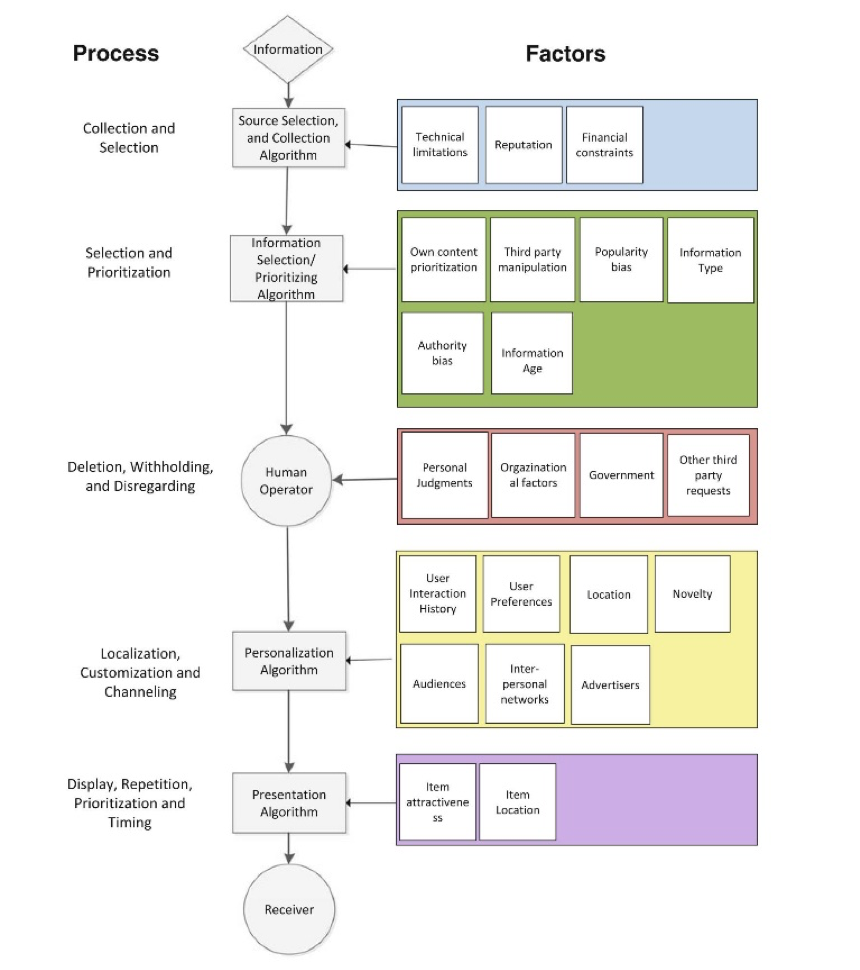
\includegraphics{img/leyer_abb1.png}
\caption{\enquote{A model of filtering for online web services including
personalization} (Bozdag 2013, S. 215)}
\end{figure}

Bereits im ersten Schritt, der Auswahl von Quellen und Sammlung von
Inhalten, werden Informationen ausgeschlossen, beispielsweise weil sie
nicht digital vorliegen oder den technischen Anforderungen des
Intermediärs nicht entsprechen. In einem zweiten Schritt wird die
Auswahl und Priorisierung von Inhalten davon bestimmt, welche Faktoren
der jeweilige Algorithmus berücksichtigt und wie er diese gewichtet.
Facebooks EdgeRank-Algorithmus priorisiert beispielsweise aktuelle
Beiträge (\emph{Information Age}) und gibt Bildern und Videos den Vorzug
vor Links und Text (\emph{Information Type}). Der Ranking-Algorithmus
von Google hingegen privilegiert eigene Produkte (\emph{Own Content
Prioritization}) und misst beliebten Inhalte größere Bedeutung zu
(\emph{Popularity Bias}).

Zudem entscheiden in einem dritten Schritt Mitarbeiter*innen der
Internet-Intermediäre (\emph{Human Operators}), ob bestimmte Inhalte
gelöscht werden -- beispielsweise um die Einhaltung der
Nutzungsbedingungen zu gewährleisten oder um auf Beschwerden von
Nutzer*innen, Rechteinhaber*innen und Regierungsorganisationen zu
reagieren. Dass diese \enquote{editorial judgments} (Bozdag 2013, S.
217) umstritten sind, zeigt beispielsweise der Skandal, den
Facebook-Mitarbei\-ter*innen durch das Löschen eines Fotos auslösten, das
zwei einander küssende Männer zeigt (Bozdag 2013).

Ob und in welcher Position Intermediäre bestimmte Inhalte anzeigen, wird
in der vierten und fünften Selektionsstufe auch von Personalisierungs-
und Präsentationsalgorithmen beeinflusst. Diese berücksichtigen nicht
nur die Interessen und das bisherige Verhalten der Nutzer*innen
(\emph{User Interaction History, User Preferences}), sondern auch deren
Standort \emph{(Location)} und Freundes-Netzwerk (\emph{Interpersonal
Networks}) sowie die Beliebtheit der Inhalte\emph{.}

Insgesamt verdeutlicht Bodzags Filter-Modell, dass sowohl die
Informationsauswahl, als auch Priorisierungs-, Personalisierungs- und
Präsentations-Entscheidungen beeinflussen, welche Inhalte an welcher
Stelle und zu welchem Zeitpunkt im Internet-Informationsintermediär
angezeigt werden.

\hypertarget{bozdags-filter-modell-anwendung-auf-selektion-in-bibliotheken}{%
\subsection{Bozdags Filter-Modell: Anwendung auf Selektion in
Bibliotheken}\label{bozdags-filter-modell-anwendung-auf-selektion-in-bibliotheken}}

Denkt man bei den einzelnen Stufen von Bozdags Modell nicht an
Internet-Intermediäre, sondern an die Erwerbungsarbeit in Bibliotheken,
fällt auf, dass die Selektionsschritte und Einflussfaktoren des Modells
ebenfalls zutreffen: Auch hier werden bereits in der ersten Stufe, der
Auswahl der Quellen, Inhalte ausgeschlossen, beispielsweise weil sie in
Deutschland nicht lieferbar sind (man denke an die Erwerbung
fremdsprachiger Bücher), weil sie zu teuer sind \emph{(Financial
Constraints}) oder -- im Falle digitaler Angebote von Öffentlichen
Bibliotheken -- vom Verlag nicht für den Verleih in Bibliotheken
freigegeben werden. Die Faktoren, die die Priorisierung bei der
Informationsauswahl in Internet-Intermediären bestimmen, treffen zum
Teil auch auf den Bestandsaufbau in Bibliotheken zu: So werden bei der
Erwerbung beispielsweise gebundene Ausgaben gegenüber
Taschenbuch-Ausgaben \emph{(Information Type)} und aktuelle Titel
bevorzugt (\emph{Information Age}). Auch ein \emph{Popularity Bias}
lässt sich im Erwerbungsmanagement der meisten Bibliotheken beobachten:
So bekommen sehr beliebte Bestandsgruppen wie zum Beispiel
Kriminalromane ein höheres Budget zugewiesen als wenig gefragte Genres
wie beispielsweise Lyrik. Auch der in Bozdags Modell zentrale
\emph{Human Operator} -- also die Erwerbungsbibliothekarin -- nimmt auf
die Auswahlentscheidungen in Bibliotheken bedeutend Einfluss.
Letztendlich entscheidet die persönliche Einschätzung der
Erwerbungsbibliothekarin, ob ein Medium für den Bestand der jeweiligen
Bibliothek notwendig und geeignet ist. Aber auch \emph{Organizational
Factors} wie beispielsweise das Leitbild einer Bibliothek, das
Bestandskonzept und die Aufteilung des Erwerbungsetats sowie die
Aufgabenverteilung unter den Mitarbeiter*innen beeinflussen, welche
Medien in den Bestand der Bibliothek aufgenommen werden.

Auch Personalisierungsprozesse -- der vierte Schritt in Bozdags Modell
-- lassen sich bei Bibliotheken beobachten. Bei der Entscheidung, ob ein
Medium für den Bestand der Bibliothek erworben wird, orientiert sich die
Erwerbungsbibliothekarin an den Zielgruppen der Bibliothek (den
\emph{Audiences}); ob und wie oft beispielsweise andere Werke zum
gleichen Thema oder der gleichen Autorin bisher ausgeliehen wurden
\emph{(User Preferences / User Interaction History}); an dem Standort
der Bibliothek, beispielsweise im Bezug auf Regionalgeschichte und
Reiseführer \emph{(Location}). Im Unterschied zum
Personalisierungs-Algorithmus in Internet-Intermediären beziehen sich
die hier aufgeführten Personalisierungsfaktoren in Bibliotheken jedoch
nicht auf einzelne Individuen, sondern auf Gruppen von Rezipient*innen.
Aber auch individuelle Personalisierung ist in Bibliotheken zu
beobachten, wenn eine Auskunftsmitarbeiterin einer langjährigen Leserin,
deren Interessen und bisheriges Ausleihverhalten sie gut kennt,
bestimmte Medien empfiehlt.

Die Präsentation von Inhalten -- der fünfte Schritt - spielt in
Bibliotheken genau wie in Internet-Intermediären eine Rolle: Medien, die
in obersten oder untersten Regalbrettern im 5. Stock der Bibliothek
aufgestellt werden, finden weniger Beachtung als frontal präsentierte
Medien in einem Neuerwerbungsregal im Erdgeschoss.

\hypertarget{das-intermediary-effects-model-wer-verursacht-verzerrungen2}{%
\subsection[Das Intermediary Effects Model: Wer verursacht
Verzerrungen?]{\texorpdfstring{Das Intermediary Effects Model: Wer
verursacht Verzerrungen?\footnote{Eine leicht veränderte Version diese
  Kapitels wurde bereits veröffentlicht (vgl. Leyrer 2018).}}{Das Intermediary Effects Model: Wer verursacht Verzerrungen?}}\label{das-intermediary-effects-model-wer-verursacht-verzerrungen2}}

Während Bozdags Modell die Einflussfaktoren in den einzelnen
Selektionsschritten innerhalb des Informationsintermediärs darstellt,
gehen Jürgens und Stark (2017) davon aus, dass Verzerrungen (sogenannte
\emph{Bias}) an unterschiedlichen Stellen -- nicht nur in den
Intermediären -- entstehen und Wirkung entfalten können. Um den Einfluss
der Internet-Informationsintermediäre zu beschreiben, reicht es daher
nicht, lediglich den Intermediär und seine Selektionsmechanismen in den
Fokus zu nehmen. Stattdessen muss die gesamte Produktions- und
Verbreitungskette von Informationen im Internet analysiert werden.
Jürgens und Stark schlagen daher ein Modell zur Analyse des Einflusses
von Intermediären vor, \enquote{that reflects the flow and manipulation
of information across different stages in the digital domain} (2017, S.
287). Dieses General Intermediary Effects Model (IEM) besteht aus drei
Selektionsschritten, die jeweils den Einfluss eines Akteurs auf den von
ihm kontrollierten Inhalt beschreiben. Als \emph{Producer} werden
Akteur*innen bezeichnet, die irgendeine Form von Inhalt generieren (zum
Beispiel Medienangebote, Nutzer*innen, Institutionen). Die
Informationsauswahl der \emph{Producer} beeinflusst die Intermediäre,
deren Informationsauswahl selbst wiederum verschiedenen
Selektionslogiken unterliegt. Die dritte Säule des Modells bilden die
Nutzer*innen, deren Informationsauswahl zwar von den Intermediären
beeinflusst wird, aber darüber hinaus auch eigenen Logiken folgt.

\begin{figure}
\centering
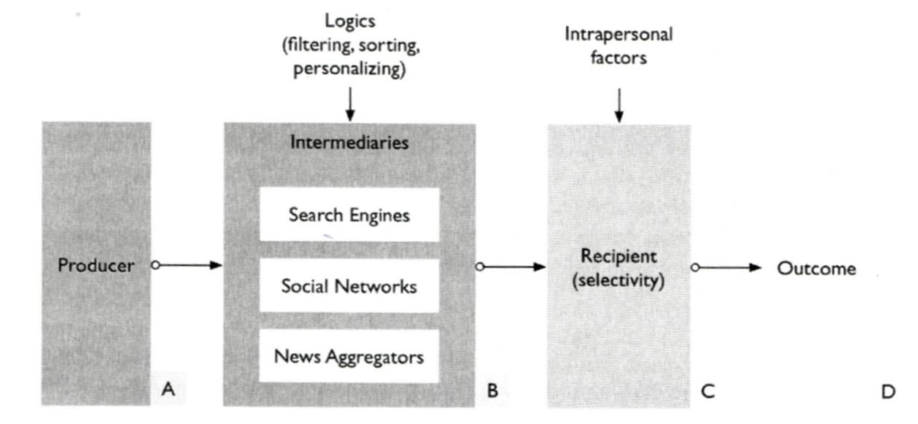
\includegraphics{img/leyer_abb2.png}
\caption{Intermediary Effects Model (Jürgens \& Stark 2017, S. 403)}
\end{figure}

Die Selektionslogiken in Internet-Intermediären können nach Jürgens und
Stark drei Formen von Verzerrungen hervorbringen: \emph{Filtering,
Sorting} und \emph{Personalization Bias}. \emph{Filtering Bias}
beschreibt, welche Inhalte gar nicht auffindbar sind oder nicht
angezeigt werden. Anders als in traditionellen Medien wie Zeitungen und
Fernsehen sind Platz beziehungsweise Sendezeit im Internet zwar nicht
begrenzt. Dennoch muss der Intermediär eine bestimmte Auswahl der im
Netz zur Verfügung stehenden Information treffen, um die Usability
seines Outputs zu gewährleisten. Eine Form von Filtering Bias ist die
Zensur, das heißt das Löschen der \enquote{expression of certain ideas}
(Jürgens \& Stark 2017, S. 399).

\emph{Sorting Bias} bedeutet, dass bestimmte Inhalte priorisiert und
somit prominenter platziert werden als andere, was dazu führt, dass sie
auch mehr Aufmerksamkeit erfahren, beispielsweise durch das Ranking von
Suchergebnissen. \emph{Personalization Bias} schließlich beschreibt die
Anpassung der Inhalte auf Basis von Informationen über die Nutzerin,
sodass jede Nutzerin ein auf sie zugeschnittenes Informationsangebot
erhält (Jürgens \& Stark 2017).

\hypertarget{anwendung-des-intermediary-effects-modells-auf-selektion-in-bibliotheken}{%
\subsection{Anwendung des Intermediary Effects Modells auf Selektion in
Bibliotheken}\label{anwendung-des-intermediary-effects-modells-auf-selektion-in-bibliotheken}}

Das Intermediary Effects Modell ist für die Einschätzung von
Verzerrungen in Bibliotheksangeboten äußerst gewinnbringend. Auch der
Einfluss von Bibliotheken auf die Auswahl der Inhalte, die Nutzer*innen
schließlich rezipieren, kann nur durch die Analyse des gesamten
Informationsflusses von den Produzent*innen bis zu den Rezipient*innen
eingeschätzt werden. Als \emph{Producer} können hier Verlage und
Medienunternehmen verstanden werden, die Bücher, Zeitschriften,
Multimedia-Angebote wie CDs, DVDs, BlueRays und Computerspiele
produzieren. Deren Informationsauswahl beeinflusst die Bibliotheken,
denn diese können nur aus dem Angebot auswählen, das ihnen auf dem
Medienmarkt zur Verfügung steht. Die Auswahl der Bibliotheken bestimmt
wiederum, welche Medien den Nutzer*innen zur Verfügung stehen; die
Nutzer*innen selbst treffen abermals eigene Auswahlentscheidungen.

Die Verzerrungsgefahr, die Jürgens und Stark bei der Selektion in
Internet-Intermediären ausmachen, lässt sich ebenfalls auf Bibliotheken
übertragen. Da Bibliotheken über begrenzte räumliche und finanzielle
Kapazitäten verfügen, gibt es Medien, die nicht zur Verfügung gestellt
werden (\emph{Filtering Bias}). \emph{Sorting Bias} entsteht durch die
Art der Medienpräsentation in den Räumen der Bibliothek, aber auch durch
das Ranking im Online-Katalog. Als \emph{Personalisation Bias} kann in
Bibliotheken schließlich die Erwerbung auf Basis von bisherigen
Ausleihzahlen, im Hinblick auf bestimmte Zielgruppen und den Standort
der Bibliothek verstanden werden. Wie oben bereits erwähnt, können auch
persönliche Empfehlungen durch das Auskunftspersonal personalisiert
erfolgen -- bewusst oder unbewusst; weil die Bibliothekarin die Leserin
kennt oder aufgrund vermuteter soziodemographischer Merkmale oder
Stilvorlieben. Dabei ist laut Kathrin Passig \enquote{der Weg zu dieser
Empfehlung unklarer als bei jedem Empfehlungsalgorithmus} (2017) -- auch
Bibliothekar*innen und Buchhändler*innen selbst können die genauen
Selektionslogiken ihrer Empfehlung nicht benennen (Passig 2017).

\hypertarget{fazit}{%
\section{Fazit}\label{fazit}}

Die modellbasierte Beschreibung der Auswahlprozesse in Bibliotheken
zeigt, dass der Aufbau, die Präsentation und die Vermittlung des
Bestandes nicht neutral erfolgen kann: Verzerrungen können in jedem der
fünf Selektionsschritte nach Bozdag entstehen. Das menschliche Gehirn
der Erwerbungs- und Auskunftsbibliothekarin ist ähnlich wie die
Selektionsalgorithmen der Internet-Intermediäre eine Black Box, sodass
eine neutrale Auswahlentscheidung in beiden Kontexten sowohl unmöglich
als auch schwer überprüfbar ist. Genauso können Verzerrungen, die auf
der Ebene von Verlagen und Medienunternehmen (also der Produzierenden
von Inhalten) entstehen, von der Bibliothek übernommen oder ausgeglichen
werden; ebenso kann auch die Auswahl der Nutzer*innen Verzerrungen
verursachen oder nivellieren.

Das bedeutet jedoch nicht, dass das Neutralitätsgebot nicht trotzdem die
Handlungsmaxime für die bibliothekarische Praxis sein muss. Es darf
jedoch nicht weiterhin ausgeklammert werden, dass es sich dabei um ein
Ideal handelt, das nicht erreichbar ist. Stattdessen muss betont werden,
dass jedes Individuum und jede Organisation \enquote{inescapable biases}
aufweisen -- nach Lankes \enquote{{[}t{]}he best one can do, from an
ethical perspective, is to disclose those biases as much as possible}
(2008).

Um Verzerrungen in Bibliotheken offenzulegen, ist es also unabdingbar,
die Selektionsmechanismen in Bibliotheken und \emph{Collection Bias}
stärker empirisch zu untersuchen. Als Basis für Forschung hierzu können
die in diesem Beitrag vorgestellten Modelle von Bozdag sowie von Jürgens
und Stark dienen.

Zudem müssen sowohl Bibliotheksmitarbeiter*innen als auch Nutzer*innen
für bewusste und unbewusste Auswahlentscheidungen beim Bestandsaufbau
und der Bestandsvermittlung sensibilisiert werden. Dazu gehört zum
Einen, die Auseinandersetzung mit Ursachen und Formen von Verzerrungen
sowie Strategien zum Umgang mit Bias in bibliothekarischen Aus- und
Fortbildungsangeboten zu verankern. Auch die Veröffentlichung und
Diskussion von empirischen Studien zu \emph{Collection Bias} in
bibliothekarischen und bibliothekswissenschaftlichen Zeitschriften und
Mailinglisten müsste die Diskussion einzelner kritischer Fragen in der
Erwerbungsarbeit ergänzen.

Zur Sensibilisierung von Nutzer*innen und Bibliotheksmitarbeiter*innen
gleichermaßen dient eine detaillierte Dokumentation und Veröffentlichung
der Erwerbungsgrundsätze der Bibliothek, in der möglichst zu allen
Einflussfaktoren der beiden hier vorgestellten Modelle Stellung bezogen
wird. Schließlich gehört es auch zur Aufgabe von Bibliotheken,
Informationskompetenz zu vermitteln und Schulungsangebote zu
Informationsauswahl und -bereitstellung im Internet zu gestalten. Dabei
liegt eine besondere Chance darin, Nutzer*innen über die
Selektionsmechanismen und Einflussfaktoren in Internet-Intermediären wie
Facebook und Google zu informieren und zugleich darauf aufmerksam
machen, dass auch Bibliotheksangebote von verschiedenen
Auswahlentscheidungen beeinflusst werden.

\hypertarget{literatur}{%
\section{Literatur}\label{literatur}}

Bozdag, Engin (2013): Bias in algorithmic filtering and personalization.
In \emph{Ethics and Information Technology} 15 (3), S.~209--227.

Flaxman, Seth; Goel, Sharad; Rao, Justin M. (2016): Filter Bubbles, Echo
Chambers, and Online News Consumption. In \emph{PUBOPQ} 80 (S1),
pp.~298--320. DOI: \url{https://doi.org/10.1093/poq/nfw006}.

Jürgens, Pascal; Stark, Birgit (2017): The Power of Default on Reddit. A
General Model to Measure the Influence of Information Intermediaries. In
\emph{Policy \& Internet} 9 (4), S.~395--419.

Lankes, R. David (2008): The Ethics of Participatory Librarianship. In
\emph{Journal of Library Administration} 47 (3-4), pp.~233--241. DOI:
\url{https://doi.org/10.1080/01930820802186555}.

Leyrer, Katharina (2018): Selektion und Bias in traditionellen und
Internet-Informations\-in\-ter\-me\-di\-ären. Forschungsstand. In: Hagenhoff,
Svenja (Hrsg.): Erlanger Beiträge zur Medienwirtschaft, 10. Online
verfügbar unter
\url{http://nbn-resolving.de/urn:nbn:de:bvb:29-opus4-102405}.

Pariser, Eli (2011): The filter bubble. What the Internet is hiding from
you. 1. publ. London: Viking.

Passig, Kathrin (2017): Fünfzig Jahre Black Box. Online verfügbar unter
\url{https://www.merkur-zeitschrift.de/2017/11/23/fuenfzig-jahre-black-box/},
zuletzt aktualisiert am 23.11.2017, zuletzt geprüft am 11.1.2018.

Quinn, Brian (2012): Collection Development and the Psychology of Bias.
In \emph{The Library Quarterly} 82 (3), pp.~277--304. DOI:
\url{https://doi.org/10.1086/665933}.

Redaktion LIBREAS (2018): CfP LIBREAS. Library Ideas \#35: Neutralität.
Bibliotheken zwischen Pluralität und~Propaganda. Online verfügbar unter:
\url{https://libreas.wordpress.com/category/libreas-call-for-papers/},
zuletzt aktualisiert am 23.11.2018, zuletzt geprüft am 1.2.2019.

Schiffler, Arne (2018): \enquote{Die Diskussion ist Ausdruck dafür, dass
die Welt ungemütlicher geworden ist.}. Online verfügbar unter
\url{https://bibliotheksnews.com/2018/06/13/die-diskussion-ist-ausdruck-dafuer-dass-die-welt-ungemuetlicher-geworden-ist/}),
zuletzt geprüft am 04.02.2019.

Stark, Birgit; Magin, Melanie; Jürgens, Pascal (2017): Ganz meine
Meinung? Informationsintermediäre und Meinungsbildung - eine
Mehrmethodenstudie am Beispiel von Facebook. Düsseldorf: Landesanstalt
für Medien Nordrhein-Westfalen (LfM-Dokumentation, Band 55).

Schleh, Bernd (2018): Schwieriger Umgang mit Büchern aus rechten
Verlagen. Online verfügbar unter
\url{https://b-u-b.de/schwieriger-umgang-rechte-verlage/}, zuletzt
aktualisiert am 13.6.2018, zuletzt geprüft am 1.2.2018.

Schulz, Wolfgang; Dankert, Kevin (2016): Die Macht der
Informationsintermediäre 2016. Erscheinungsformen, Strukturen und
Regulierungsoptionen. Bonn: Friedrich-Ebert-Stiftung.

Schweiger, Wolfgang (2017): Der (des)informierte Bürger im Netz.
Wiesbaden: Springer Fachmedien Wiesbaden.

Tewksbury, David; Rittenberg, Jason (2012): News on the internet.
Information and citizenship in the 21st century. New York, N.Y.: Oxford
University Press (Oxford studies in digital politics).

%autor
\begin{center}\rule{0.5\linewidth}{\linethickness}\end{center}

\textbf{Katharina Leyrer} ist seit 2018 Wissenschaftliche Mitarbeiterin
und Doktorandin am Institut für Buchwissenschaft. Ihr Studium der
Bibliotheks- und Informationswissenschaft in Leipzig, Berlin und Lyon
schloss sie 2017 mit Förderung der Heinrich-Böll-Stiftung ab. Danach war
sie in der Stadtbibliothek Erlangen und als Lehrbeauftragte an der HTWK
Leipzig tätig. Ihre Forschungsinteressen liegen bei der Wechselwirkung
von Digitalisierung und Gesellschaft, insbesondere bei Privatsphäre und
Meinungsbildung im Netz, sowie bei Digitalen Bibliotheken. Sie lehrt in
den Studiengängen Digital Humanities und Buchwissenschaft.

\end{document}
